%!TEX root = ../report.tex
%\cleardoublepage
%\clearpage
%
%\appendix
%\appendixpage
%\addappheadtotoc

\begin{appendices}
			
	%\addcontentsline{toc}{part}{\appendixname}
				
	\renewcommand{\thechapter}{\Alph{chapter}}
	\renewcommand{\thesection}{\thechapter.\arabic{section}}
	\renewcommand{\thesubsection}{\thesection.\arabic{subsection}}
	\renewcommand{\thesubsubsection}{\thesubsection.\arabic{subsubsection}}
	
	\chapter{Requirements}
	\section{Usecases}
	This section elaborates the architectural important use-cases using tables.
	
	\subsection{Receive weather/GEO/demographic data}
	\begin{table}[H]
	\pgfplotstabletypeset[%
		UCTable
	]{%
		value & description \\
		Number & \req{uc}\\
		Description & The system receives data from the weather forecast service, the geographic API and the demographic API \\
		Stakeholders and interests & 
		\textbf{Third Party}, \textbf{Safety Region} and \textbf{Citizens}: They want to receive accurate warnings about floods. \\
		Primary actor & System (timer)\\
		Scope & Monitoring part of the system \\
		Level & Sub process\\
		Precondition & There is a connection between the API and our system \\
		Main success scenario & \compactList{enumerate}{%
			\item The processing unit determines it needs external data%
			\item A call is made to the relevant external API%
			\item The external API returns the requested data
			}\\
		Postcondition & The system received the external data \\
		Alternatives & \compactList{itemize}{%
			\item[3a.] 
			\begin{enumerate}
				\item The data cannot be returned.
				\item Repeat this process with another external API service.
				\item If none are available, proceed monitoring without the requested external data.
				\item After 5 minutes try to reconnect.
			\end{enumerate}
			}\\
		Related requirements & \ref{fr:receive-weather}, \ref{fr:receive-geographic}, \ref{fr:receive-demographic}, \ref{fr:compute-nrcivilians}\\
	}
	\caption{UC-\arabic{uc}: Receive weather/GEO/demographic data}
	\label{table:uc-receive-weathergeo}
	\end{table}

	\clearpage
	\subsection{Subscribing to SMS Service}
	\begin{table}[H]
	\pgfplotstabletypeset[%
		UCTable
	]{%
		value & description \\
		Number & \req{uc}\\
		Description & Citizens can subscribe to the SMS service, so when a flood is imminent they will receive a text message\\	
		Stakeholders and interests & 
		\textbf{Citizens}: Citizens want to be warned as soon as possible.
		\\
		Primary actor & Citizen\\
		Scope & Warning part of the system \\
		Level & User goal \\
		Precondition & Citizen has a connected mobile phone and is not subscribed to the SMS service \\
		Main success scenario & \compactList{enumerate}{
			\item Citizen sends a text message containing his/her address information to our SMS service
			\item The SMS service receives the text message
			\item The SMS service sends the phone number and address data to the SFM system
			\item The SFM system stores the phone number and address in the database
			\item A text message is sent back to the citizen with confirmation by the SMS service
			}\\
		Postcondition & Citizen is subscribed to the SMS service \\
		Alternatives & \compactList{itemize}{%
			\item[2a.] 
			\begin{enumerate}
				\item The text message is not received \\
				\item The use-case ends, the user has no confirmation text and should resend his/her text message
			\end{enumerate}
			}\\
		Related requirements & \ref{fr:citizens-subscribe} \\
	}
	\caption{UC-\arabic{uc}: Subscribing to SMS Service}
	\label{table:uc-sms-service}
	\end{table}

	\clearpage
	\subsection{Determining flood probability}
	\begin{table}[H]
	\pgfplotstabletypeset[%
		UCTable
	]{%
		value & description \\
		Number & \req{uc}\\
		Description & The central processing unit calculates the probability of a flood \\
		Stakeholders and interests & \compactCell{
			\textbf{Safety region}: The safety region wants to know when a flood warning is triggered \\
			\textbf{Citizens}: The citizens want to be alerted if there is a high enough probability of a flood occurring \\
			\textbf{Third Parties}: Third Parties want to have access to the flood probability data}
			\\
		Primary actor & System (timer) \\
		Scope & Monitoring part of the system \\
		Level & Sub process\\
		Precondition & The sensor/geographic/weather data is available \\
		Main success scenario & \compactList{enumerate}{%
			\item The central processing unit gets the latest sensor data from the database
			\item The central processing unit gets the latest weather/geographic data
			\item The central processing unit calculates the probability of a flood
			\item The central processing unit stores the probability value in the database
			\item The central processing unit determines that a flood is imminent based on the probability value
			\item The central processing unit invokes the warning part of the system
			\item A UAV is dispatched to the area where the flood is
			\item During the flood, the UAV provides imagery data of the flood area
			}\\
		Postcondition & The flood probability is calculated and stored. If the flood was imminent, the warning part was invoked. \\
		Alternatives & \compactList{itemize}{
			\item[5a.] 
			\begin{enumerate}
			  \item The probability is not above the threshold
			  \item The use-case ends
			\end{enumerate}
			\item[5b.]
			\begin{enumerate}
			  \item The system cannot determine with enough certainty there is a flood
			  \item A UAV is dispatched to check
			\end{enumerate}
			}\\
		Related requirements & \ref{fr:detect-flood}, \ref{fr:uav}, \ref{fr:uavflood}, \ref{fr:uavprocessflood} \\
	}
	\caption{UC-\arabic{uc}: Determining flood probability}
	\label{table:uc-determine-flood-probability}
	\end{table}

	\clearpage
	\subsection{Warn citizens}
	\begin{table}[H]
	\pgfplotstabletypeset[%
		UCTable
	]{%
		value & description \\
		Number & \req{uc}\\
		Description & Citizens who are subscribed to the SMS service will be warned through text messages in case of an imminent flood\\	
		Stakeholders and interests & 
			\textbf{Citizens}: When they are subscribed, they want to be warned in case of an imminent flood
			\\
		Primary actor & Citizen\\
		Scope & Warning part of the system \\
		Level & User goal \\
		Precondition & \compactList{enumerate}{
		\item There is an imminent flood 
		\item The citizen is subscribed to the SMS service}\\
		Main success scenario & \compactList{enumerate}{%
			\item The flood monitoring \& detection unit sends a warning about an imminent flood to the warning unit
			\item The warning unit queries the database for a list of phone numbers of subscribed citizens in the area
			\item The warning unit sends the collected phone numbers to the SMS service
			\item The SMS service sends a warning to all the collected phone numbers
			}\\
		Postcondition & The citizens who are subscribed received a warning\\
		Alternatives & \compactList{itemize}{%
			\item[3a.] 
			\begin{enumerate}
				\item A message cannot be sent to the citizen
				\item Wait a minute and resend
				\item The use-case ends
			\end{enumerate}
			}\\
		Related requirements & \ref{fr:warn-citizens} \\
	}
	\caption{UC-\arabic{uc}: Warn citizens}
	\label{table:uc-warn-citizens}
	\end{table}

	\clearpage
	\subsection{Warn safety region}
	\begin{table}[H]
	\pgfplotstabletypeset[%
		UCTable
	]{%
		value & description \\
		Number & \req{uc}\\
		Description & The safety region needs to receive a warning about an imminent flood\\
		Stakeholders and interests & 
			\textbf{Safety regions}: The emergency services want to help the citizens in case of a flood
			\\
		Primary actor & Safety region \\
		Scope & Warning part of the system \\
		Level & User goal \\
		Precondition & There is an imminent flood\\
		Main success scenario & 
		\compactList{enumerate}{
			\item The processing unit determines what area will be under water in case of a flood
			\item The processing unit determines how many people will be affected by the imminent flood
			\item The processing unit predicts how the flood will develop in the following period 
			\item The processing unit sends a warning to the safety region
			}
			\\
		Postcondition & A warning about the flood has been send to the safety region \\
		Alternatives &  \\
		Related requirements & \ref{fr:compute-area}, \ref{fr:analyze-waterlevel}, \ref{fr:estimate-waterlevel}, \ref{fr:compute-nrcivilians}, \ref{fr:warn-safetyregion} \\
	}
	\caption{UC-\arabic{uc}: Warn safety region}
	\label{table:uc-warn-safetyregion}
	\end{table}

	\clearpage
	\subsection{Allow 3rd party access to data (API)}
	\begin{table}[H]
	\pgfplotstabletypeset[%
		UCTable
	]{%
		value & description \\
		Number & \req{uc}\\
		Description & Third parties can use the API exposed by the flood monitoring system in third party applications (providing guidance to citizens) \\
		Stakeholders and interests & \compactCell{
			\textbf{Third parties}: Third parties want to access the data of the flood monitoring system to use in their applications \\
			\textbf{Citizens}: Citizens want to receive guidance in case of a flood \\}
			\\
		Primary actor & Third party \\
		Scope & The API part of the system \\
		Level & User goal \\
		Precondition & The third party has access to the flood monitoring systems API \\
		Main success scenario & \compactList{enumerate}{
			\item The third party application connects to the API
			\item The third party application sends a request for certain data to the API
			\item The system retrieves the requested data from the database
			\item The system sends the retrieved data to the third party application
			}\\
		Postcondition & The third party application has received the requested data \\
		Alternatives &  \compactList{itemize}{
			\item[1a.] 
			\begin{enumerate}
				\item The third party cannot connect to the API
				\item The use-case ends
			\end{enumerate}
			}\\
		Related requirements & \ref{fr:expose-api} \\
	}
	\caption{UC-\arabic{uc}: Third party accessing data through the systems API}
	\label{table:uc-thirdparty-api}
	\end{table}

	\clearpage
	\subsection{Detecting a faulty sensor}
	\label{subsec:detecting-faulty-sensor}
	\begin{table}[H]
	\pgfplotstabletypeset[%
		UCTable
	]{%
		value & description \\
		Number & \req{uc}\\
		Description & The system is able to detect when a sensor is not functioning properly \\
		Stakeholders and interests & \compactCell{
			\textbf{Product owner}: The product owner wants the system to be reliable and errors/broken sensors to be fixed \\
			\textbf{Maintainers}: The maintainers are responsible for repairing/replacing the faulty sensors}
			\\
		Primary actor & The system \\
		Scope & The monitoring part of the system \\
		Level & Sub process \\
		Precondition & The sensor is not functioning properly \\
		Main success scenario & \compactList{enumerate}{
			\item The system receives the sensor data
			\item The system compares the sensor data with other information, like data of nearby sensors previous data of this sensor 
			\item The system detects that this reading is abnormal, but determines it cannot be caused by an (imminent) flood
			\item The system ignores further readings from this sensor and reports the faulty sensor in the control panel
			}\\
		Postcondition & The faulty sensor is not used in future measurements and is reported in the control panel \\
		Alternatives & \compactList{itemize}{%
			\item[3a.] 
			\begin{enumerate}
				\item The system cannot determine the abnormal reading is not caused by a flood
				\item The system will dispatch a UAV to check for a flood
				\item The system keeps using this sensors data, until it can determine that the readings are not caused by a flood, or it determines that it is caused by a flood (in which case it will issue warnings, see \hyperref[uc:4]{UC-4})
			\end{enumerate}
			\item [1a.]
			\begin{enumerate}
			    \item The system does not receive any data from the sensor for 10 minutes %TODO: discuss on friday
			    \item The system reports the faulty sensor in the control panel
			\end{enumerate}
			}\\
		Related requirements & \ref{fr:detect-faultysensor}, \ref{fr:report-faultysensors}, \ref{fr:controlpanel-warnings}, \ref{fr:controlpanel-errors}, \ref{fr:controlpanel-sensors}, \ref{fr:uavfaulty}, \ref{fr:uavprocessfaulty}
		\\
	}
	\caption{UC-\arabic{uc}: Detecting a faulty sensor}
	\label{table:uc-detect-faultysensor}
	\end{table}

	\clearpage
	\subsection{Checking the system state}
	\begin{table}[H]
	\pgfplotstabletypeset[%
		UCTable
	]{%
		value & description \\
		Number & \req{uc}\\
		Description & A maintainer of the system regularly checks the state of the system in the control panel to see if there are errors or sensors that need maintenance. \\
		Stakeholders and interests & 
			\textbf{Maintainer}: The maintainer wants to detect errors in the system in a reliable and simple way.
			\\
		Primary actor & Maintainer \\
		Scope & The maintenance part of the system \\
		Level & User goal \\
		Precondition &  \\
		Main success scenario & \compactList{enumerate}{
			\item The maintainer uses his/her login credentials to get access to the control panel
			\item The maintainer navigates to the errors/warning page
			\item The maintainer checks on this page if there are problems with the system (errors/warning)
			\item The maintainer takes necessary action to resolve any issues
			}\\
		Postcondition & The maintainer is aware of reported problems with the system \\
		Alternatives &  \\
		Related requirements & \ref{fr:controlpanel}, \ref{fr:report-faultysensors}, \ref{fr:controlpanel-warnings}, \ref{fr:controlpanel-errors}, \ref{fr:controlpanel-sensors} \\
	}
	\caption{UC-\arabic{uc}: Maintenance employee checks system state}
	\label{table:uc-maintanance-check-state}
	\end{table}

	\chapter{Hardware Architecture}
	\section{Server Specification}
	% Probably move this into appendix
	\begin{table}[!htbp]
	    \centering
	    \begin{tabular}{L{\tw{0.2}} L{\tw{0.4}}}
	    \toprule
	    \multicolumn{2}{c}{Dell PowerEdge R530 Specification} \\ \midrule
	    \textbf{Item Description} & Dell PowerEdge R530 - E5-2620V3 Xeon 2.4 GHz - 16 GB - 1 TB \\
	    \textbf{Type} & Server - rack-mountable \\
	    \textbf{Height (Rack Units)} & 2U \\
	    \textbf{Processor} & 1 x Intel Xeon E5-2620V3 / 2.4 GHz (3.2 GHz) (6-core) \\
	    \textbf{Processor Main Features} & Intel Turbo Boost Technology 2 \\
	    \textbf{Cache Memory} & 15 MB \\
	    \textbf{Cache per processor} & 15 MB \\
	    \textbf{RAM} & 16 GB (installed) / 384 GB (max.) - DDR4 SDRAM - 2133 MHz \\
	    \textbf{Storage Controller} & RAID (SATA 6Gb / s) (Dell PERC H330) \\
	    \textbf{Optical Storage} & DVD burner \\
	    \textbf{Graphics Controller} & Matrox G200 \\
	    \textbf{Video Memory} & 16 MB \\
	    \textbf{Network} & GigE \\
	    \textbf{Dimensions} &  (WxDxH)48.24 cm x 64.6 cm x 8.68 cm \\
	    \textbf{Weight} & 2.14 kg \\
	    \bottomrule
	    \end{tabular}
	\caption{Hardware specification of Dell PowerEdge R530}
	\label{table:server-specs}
	\end{table}
	
	\chapter{Software Architecture}
	\section{Database diagram}
	\begin{figure}[H]
		\centering
		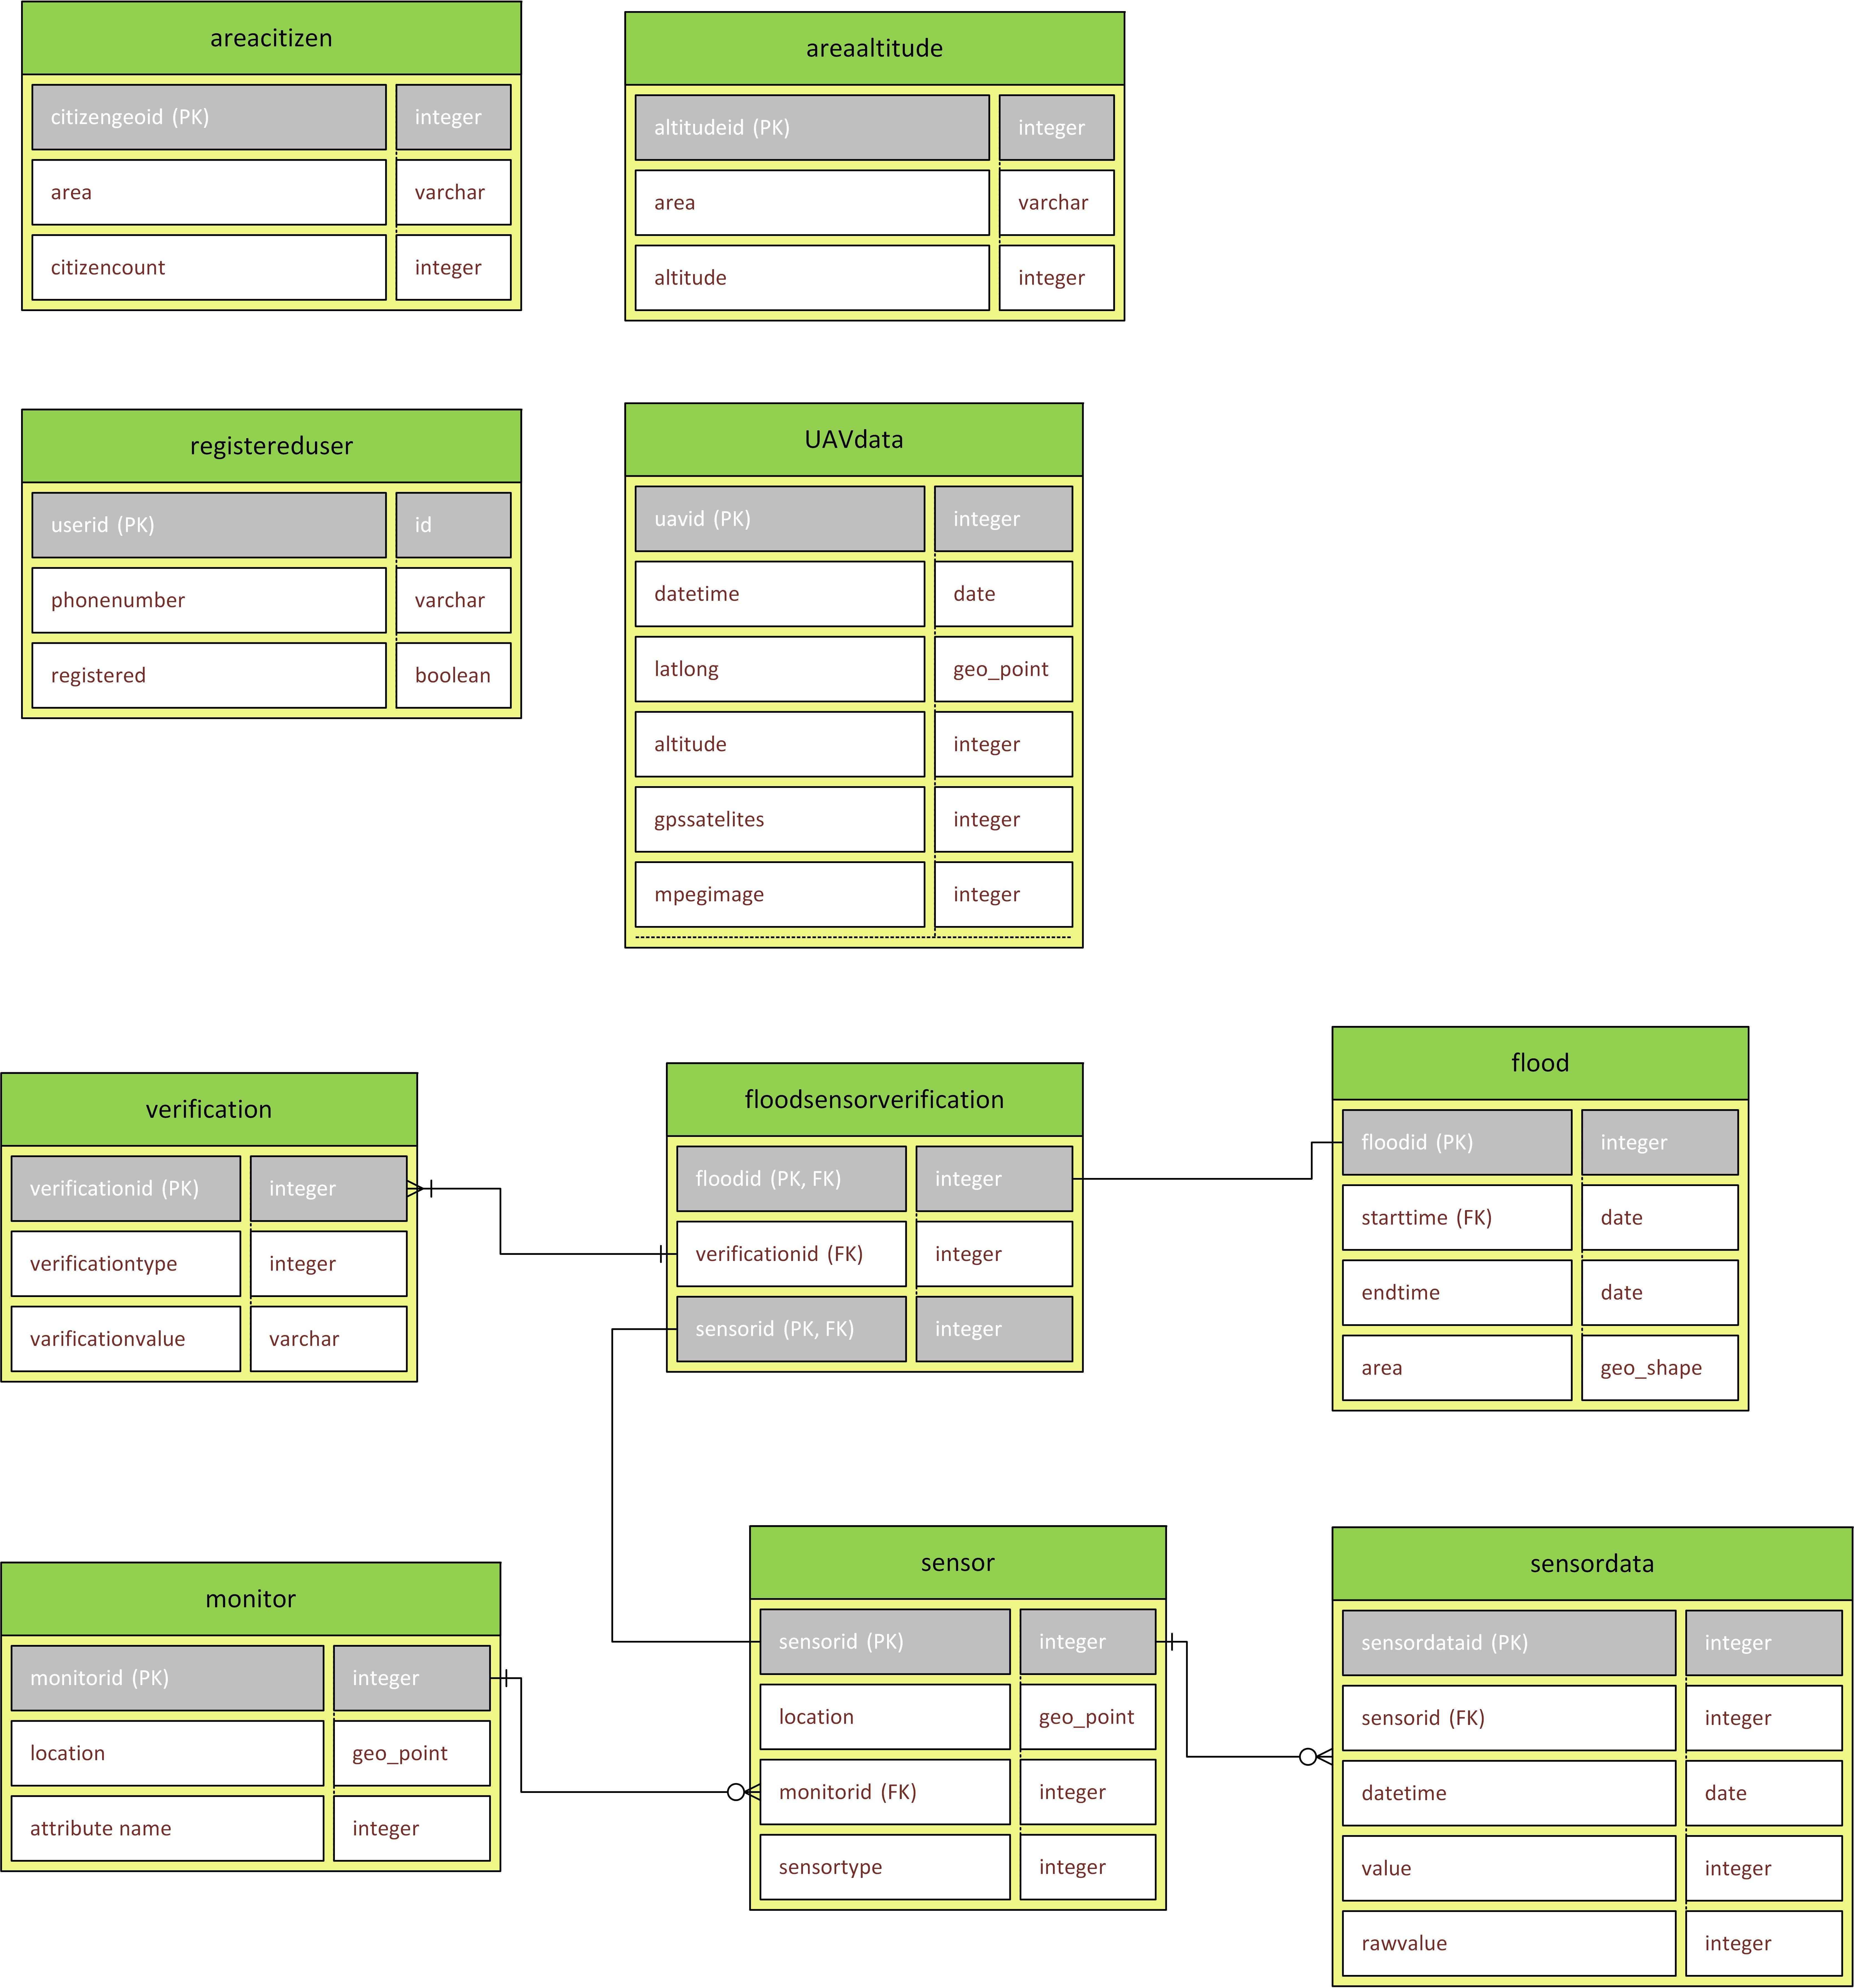
\includegraphics[height=14cm, width=0.9\textwidth]{{\viewimages/database}.jpg}
		\caption{Database diagram}
		\label{fig:database}
	\end{figure}

	% \afterpage{
	\begin{landscape}
	\section{Activity diagram}
	\begin{figure}[H]
		\centering
		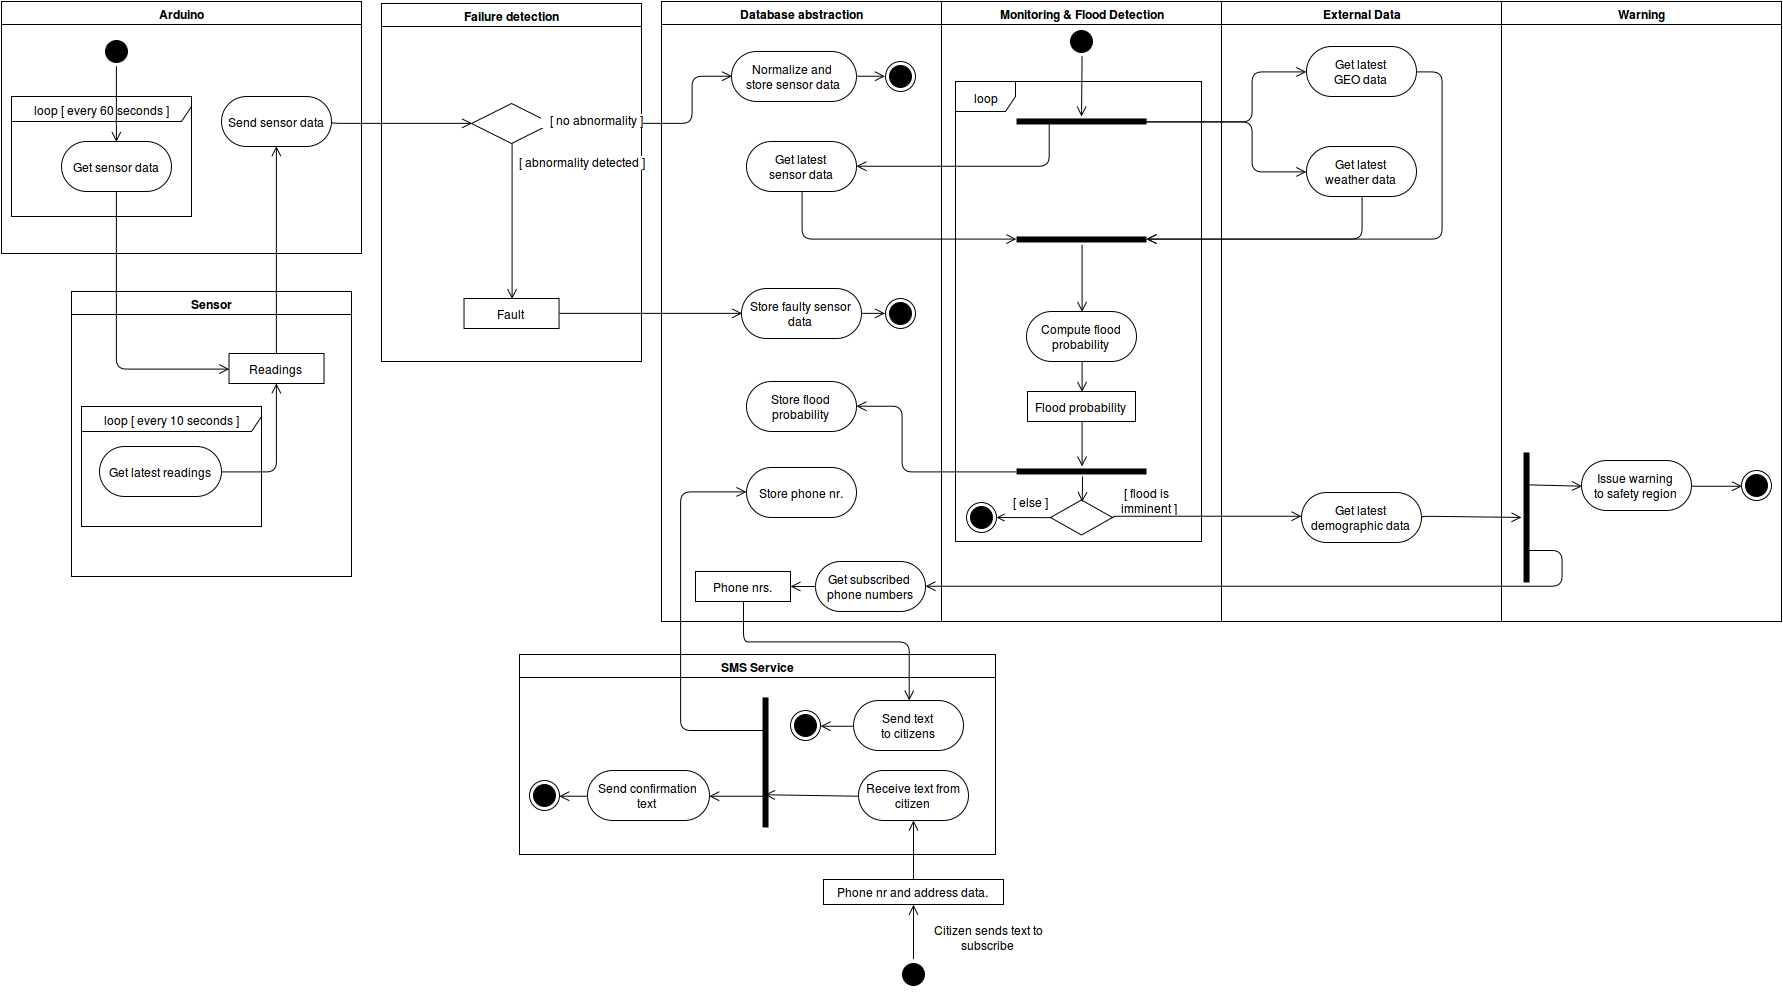
\includegraphics[keepaspectratio=true,width=1.0\textwidth]{{\viewimages/activity_monitoring}.png}
		\caption{An activity diagram of the flood monitoring process}
		\label{fig:activity-monitoring}
	\end{figure}
	% \end{landscape}
	% }
	
	% \afterpage{
	% \begin{landscape}
	\section{Deployment diagram}
	\begin{figure}[H]
		\centering
		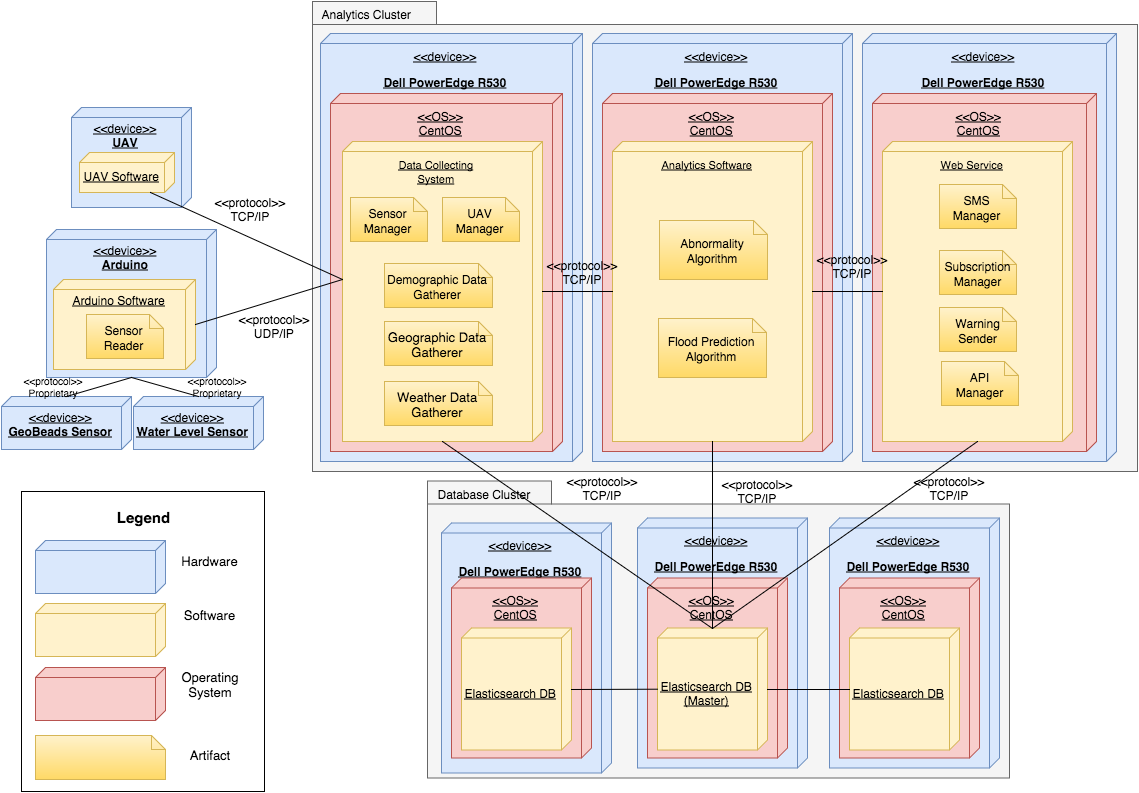
\includegraphics[keepaspectratio=true,width=0.8\textwidth]{{\viewimages/deployment-view}.png}
		\caption{Deployment diagram}
		\label{fig:deployment-diagram}
	\end{figure}
	\end{landscape}
	% }\clearpage

	%!TEX root = ../report.tex
\chapter{Time Tracking}
\label{App: Time Tracking}

%\section{Week #}
%\begin{tabular}{p{0.2\textwidth} p{0.7\textwidth} p{0.1\textwidth}}
%    \textbf{Person} & \textbf{Task} & \textbf{Hours} \\ \midrule
%	Eedema &  &  \\ \midrule
%	Putra &  &  \\ \midrule
%	Fakambi & & \\ \midrule
%	Schaefers &  & \\ \midrule
%	Brandsma &  & \\ \midrule
%	Menninga &  &  \\ \midrule
%\end{tabular}

\section{Week 1}
\begin{tabular}{L{0.2\textwidth} L{0.7\textwidth} L{0.1\textwidth}}
    \textbf{Person} & \textbf{Task} & \textbf{Hours} \\ \toprule
	Eedema & Reviewing the document, reading the assignment, initializing requirements, \& installing environment for project & 8 \\ \midrule
	Putra & Initial preparation for the course & 5 \\ \midrule
	Fakambi & Reading the document and assignment, Preparation and drafts with ideas & 5 \\ \midrule
	Schaefers & Setting up the working environment, create the context page and analysis page drafts. Setting up and improving the the document structure. & 8\\ \midrule
	Klinkenberg & & \\ \midrule
	Brandsma & Creating working environment, reading assignment, first draft business part & 8\\ \midrule
	Menninga & Reading assignment, setting up working environment, first non-functional requirements & 5 \\ \bottomrule
\end{tabular}

\section{Week 2}
\begin{tabular}{L{0.2\textwidth} L{0.7\textwidth} L{0.1\textwidth}}
    \textbf{Person} & \textbf{Task} & \textbf{Hours} \\ \toprule
	Eedema & Coaching session, project planning session and work on business information chapters & 9  \\ \midrule
	Putra & Coaching session, project planning session, project meeting, first version of stakeholder part of requirements & 7.5 \\ \midrule
	Fakambi & Coaching session , project meeting, work on Non functional requirements & 7 \\ \midrule
	Schaefers & First coaching session, improved and enhanced the context and business information chapters. Also created a quality attributes prioritization table.& 8 \\ \midrule
	Klinkenberg & Coaching session, meetings, providing feedback on requirements & 5.5\\ \midrule
	Brandsma & First version of use-cases, coaching session, meeting, use-cases, architectural vision & 6.5 \\ \midrule
	Menninga & First version of the functional requirements, coaching session, meeting & 10.25 \\ \bottomrule
\end{tabular}

\section{Week 3}
\begin{tabular}{p{0.2\textwidth} p{0.7\textwidth} p{0.1\textwidth}}
   \textbf{Person} & \textbf{Task} & \textbf{Hours} \\ \midrule
	Eedema &  Coaching, meetings, analysis, business part, reviewing & 14  \\ \midrule
	Putra & Coaching session, meetings, proofread on chapter 1 and 2, revising stakeholders, database decision part of analysis, and preparing \LaTeX{} file for the presentation & 10 \\ \midrule
	Fakambi & Coaching session, meetings, Non functional requirements and Risk assessment & 10.5\\ \midrule
	Schaefers & Coaching session, meetings, reviewing, Business section & 12 \\ \midrule
	Klinkenberg & Coaching session, meetings, technical requirements, analysis, reviewing & 13.5 \\ \midrule
	Brandsma & Coaching session, meeting, architectural vision, use-cases, analysis & 9 \\ \midrule
	Menninga & Coaching session, meetings, updates functional requirements, reviewing entire document, updated assumptions and some improvements to structure of analysis, added decision about type of water level sensor. & 14.0 \\ \midrule
\end{tabular}

\section{Week 4}
\begin{tabular}{p{0.2\textwidth} p{0.7\textwidth} p{0.1\textwidth}}
   \textbf{Person} & \textbf{Task} & \textbf{Hours} \\ \midrule
	Eedema & Coaching session, meetings, business chapter, review 3, presentations, peer review &13  \\ \midrule
	Putra & Coaching session, meetings, presentation prep., improving business rationale, review chapter 2, making draft of chapter 5, 6, and 7 & 14 \\ \midrule
	Fakambi & Coaching session , meetings , Work on and improvements chapter 3.5 to 3.8 & 12 \\ \midrule
	Schaefers & Researched on sensors and other EWS's. Then created the system architecture model diagram and vision diagram for the presentation I had to present in. Created/improved other diagrams. Researched about the costs of these kinds of systems and created/enhanced the business cost section. & 20 \\ \midrule
	Brandsma & Coaching session, meetings , reviewing group 1, architectural vision, use-cases, reviewing, improving chapter 4 & 16.5\\ \midrule
	Menninga & Coaching session, presentation prep., meeting, improvements FR and risks, review ch. 4, improvements to NFR and Risk Assessment & 14.0 \\ \midrule
\end{tabular}

\section{Week 5}
\begin{tabular}{p{0.2\textwidth} p{0.7\textwidth} p{0.1\textwidth}}
    \textbf{Person} & \textbf{Task} & \textbf{Hours} \\ \midrule
	Eedema & Coaching meetings, reviewing, chpt 5  & 13 \\ \midrule
	Putra & Coaching session, meetings, reviewing, working on initial work on chapter hardware, researching on servers, and working on server selection  & 15 \\ \midrule
	Fakambi & Coaching session, meetings, Work on chapter 6 Hardware architecture, drafts, design decision about UAVs & 12.0 \\ \midrule
	Schaefers & Created initial layer diagram, component diagram, sequense diagram and database design diagram. Researched and explained what new database to use.  & 15\\ \midrule
	Brandsma & Coaching session, meetings, chapter 5  & 13 \\ \midrule
	Menninga & Coaching session, meeting Tuesday, lots of improvements to chapter 3, expanding chapter 6 & 15.5 \\ \midrule
\end{tabular}

\section{Week 6}
\begin{tabular}{p{0.2\textwidth} p{0.7\textwidth} p{0.1\textwidth}}
    \textbf{Person} & \textbf{Task} & \textbf{Hours} \\ \midrule
	Eedema & Coaching, meetings, review, system overview, evaluation & 15 \\ \midrule
	Putra & Coaching session, meetings, reviews, hardware overview, deployment view & 13 \\ \midrule
	Fakambi & Coaching session, meetings, Work on chapter 6 Hardware architecture, drafts, design decision about UAVs, draft about chapter 7 & 9 \\ \midrule
	Schaefers & Meetings. Worked on the implementation and logical section of the software chapter. & 13 \\ \midrule
	Brandsma & &  \\ \midrule
	Menninga & Coaching session, meetings, reviews, hardware overview (sensors)/costs, implementation view, process view & 13.0 \\
	\midrule
\end{tabular}
	% %!TEX root = ../report.tex
\chapter{Todo} % (fold)
\label{sec:todo}
\todo[inline]{Create figure with processflow and place it somewhere logical}
% section todo (end)
\end{appendices}